\documentclass[aspectratio=169]{beamer}

%%%%%%%%%%%%%%%%%%%%%%%%%%%%%%%%%%%%%%%%
%% Paquetes
\input{formatoBeamerPUCE}
\usepackage{tikz}

\usetikzlibrary{arrows}
\usetikzlibrary{matrix, positioning}
\usetikzlibrary{calc}

\usepackage{qrcode}

%%%%%%%%%%%%%%%%%%%%%%%%%%%%%%%%%%%%%%%%
%% Datos
\title{Reconocimiento automático de imágenes para reconstrucción de redes planta-polinizador}
\author{Andrés Merino T.}
\date{Abril 2025}
\institute{Facultad de Ciencias Exactas, Naturales y Ambientales}

\begin{document}

%%%%%%%%%%%%%%%%%%%%%%%%%%%%%%%%%%%%%%%%
%% Página de título

\fondo{inicio}
\begin{frame}[plain]
    \vspace*{0.85cm}
    \addtocounter{framenumber}{-1}
    \hspace*{0.6cm}
    \begin{minipage}[t]{\dimexpr\textwidth-1cm}
        \titlepage
    \end{minipage}
\end{frame}


%%%%%%%%%%%%%%%%%%%%%%%%%%%%%%%%%%%%%%%%
%% Página de índice
\fondo{blanco}
\begin{frame}
    \frametitle{Contenido}
    \vspace*{-0.5cm}

    \tableofcontents
\end{frame}

%%%%%%%%%%%%%%%%%%%%%%%%%%%%%%%%%%%%%%%%
%% Secciones
% --- Parte divulgativa ---
%%%%%%%%%%%%%%%%%%%%%%%%%%%%%%%%%%%%%%%%%%%%%%%%%%%%%%%%
\fondo{celeste}
\section{Motivación}
\fondo{blanco}
%%%%%%%%%%%%%%%%%%%%%%%%%%%%%%%%%%%%%%%%%%%%%%%%%%%%%%%%

%%%%%%%%%%%%%%%%%%%%%%%%%%%%%%%%%%%%%%%%%%%%%%%%%%%%%%%%
\begin{frame}{¿Cuál es más fácil?}
    \begin{columns}[c]

    \column{.2\textwidth}
    \begin{block}{Opción A}
        \centering\vspace{0.4cm}
        {\large $6 \times 2$}
        \vspace{0.4cm}
    \end{block}


    \column{.79\textwidth}
    \begin{block}{Opción B}
        \centering
        {\small ¿En cuál imagen hay una \textit{Pristimantis croceoinguinis}?}\\[0.3cm]
        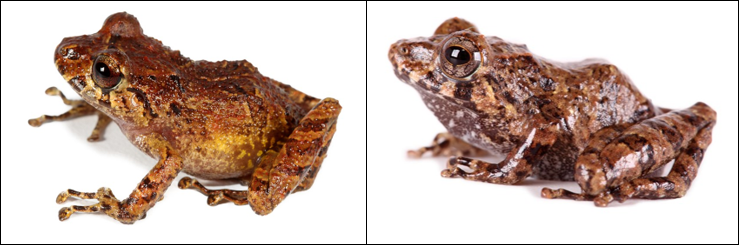
\includegraphics[width=\linewidth]{Figuras/cutin.png}
    \scriptsize Foto: Santiago Ron-BIOWEB, https://bioweb.bio.
    \end{block}
    \end{columns}
\end{frame}
%%%%%%%%%%%%%%%%%%%%%%%%%%%%%%%%%%%%%%%%%%%%%%%%%%%%%%%%

%%%%%%%%%%%%%%%%%%%%%%%%%%%%%%%%%%%%%%%%%%%%%%%%%%%%%%%%
\begin{frame}{¿Cuál es más fácil?}
    \begin{columns}[c]

    \column{.24\textwidth}
    \begin{block}{Opción A}
        \centering\vspace{0.25cm}
        {\small
            $695\,951$\\[2pt]
            $\times\ 154\,465\,122$\\[2pt]
            $\times\ 111\,154\,465.122$\\[2pt]
            $\times\ 1\,514\,616\,454\,651$
        }
        \vspace{0.3cm}
    \end{block}

    \column{.74\textwidth}
    \begin{block}{Opción B}
        \centering
        {\small ¿En cuál imagen hay un perro?}\\[0.3cm]
        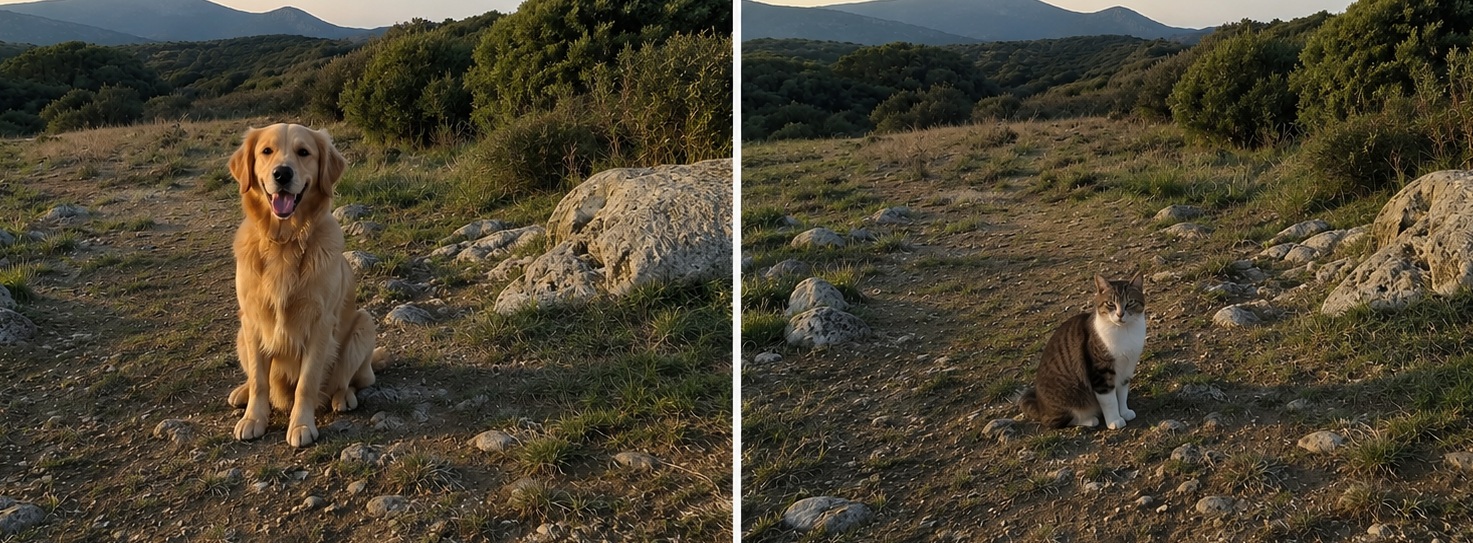
\includegraphics[width=\linewidth]{Figuras/perro02.png}
    \end{block}
    \end{columns}
\end{frame}
%%%%%%%%%%%%%%%%%%%%%%%%%%%%%%%%%%%%%%%%%%%%%%%%%%%%%%%%

%%%%%%%%%%%%%%%%%%%%%%%%%%%%%%%%%%%%%%%%%%%%%%%%%%%%%%%%
\fondo{celeste}
\section{¿Qué es una imagen?}
\fondo{blanco}
%%%%%%%%%%%%%%%%%%%%%%%%%%%%%%%%%%%%%%%%%%%%%%%%%%%%%%%%

%%%%%%%%%%%%%%%%%%%%%%%%%%%%%%%%%%%%%%%%%%%%%%%%%%%%%%%%
\begin{frame}
    \frametitle{¿Qué es una imagen?}
    \begin{block}{}
        Una imagen digital se representa como una matriz de valores, donde cada elemento (píxel) de la matriz almacena la intensidad de luz en un punto específico de la imagen.
    \end{block}

\begin{center}
    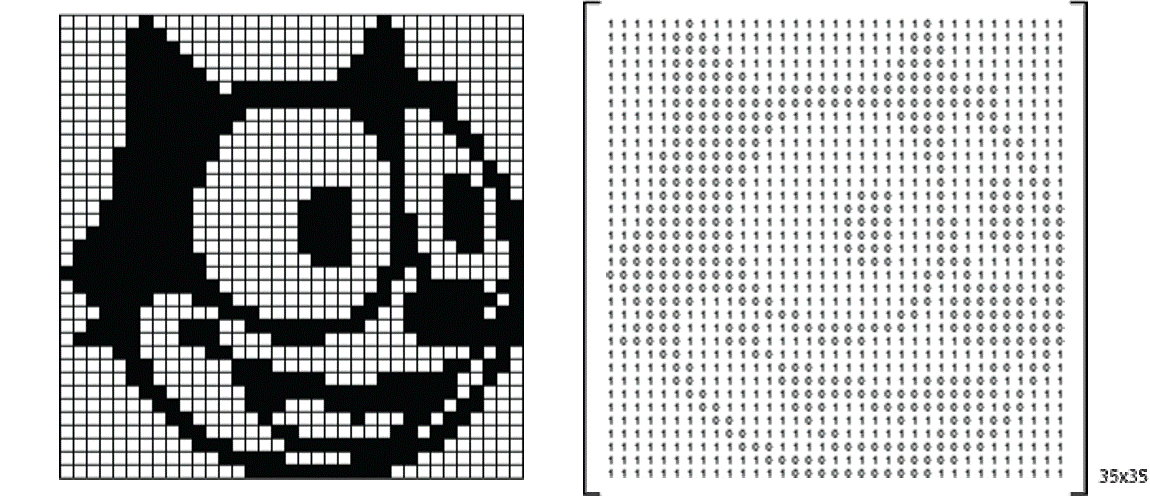
\includegraphics[width=9.5cm]{Figuras/Img01}
\end{center}


\end{frame}
%%%%%%%%%%%%%%%%%%%%%%%%%%%%%%%%%%%%%%%%%%%%%%%%%%%%%%%%

%%%%%%%%%%%%%%%%%%%%%%%%%%%%%%%%%%%%%%%%%%%%%%%%%%%%%%%%
\begin{frame}{El formato RGB}
    \begin{columns}
    \column{.5\textwidth}
    \begin{itemize}
        \item 
        Modelo de color basado en la síntesis aditiva
        \item 
        Es posible representar un color mediante la mezcla por adición de los tres colores de luz primarios: \textcolor{red}{rojo}, \textcolor{green}{verde} o \textcolor{azul}{azul}.
        \item 
        Tiene rangos de 0 a 255 (enteros) o de 0 a 1 (reales).
    \end{itemize}
    \column{.5\textwidth}
        \postitimg[6cm]{Figuras/Img02} % Inserta la figura correspondiente
    \end{columns}
\end{frame}
%%%%%%%%%%%%%%%%%%%%%%%%%%%%%%%%%%%%%%%%%%%%%%%%%%%%%%%%

%%%%%%%%%%%%%%%%%%%%%%%%%%%%%%%%%%%%%%%%%%%%%%%%%%%%%%%%
\begin{frame}{Ejemplo}
    \[
        R = \begin{pmatrix}
            0.0& 0.3& 0.9\\
            1.0& 0.0& 1.0
        \end{pmatrix};\quad
        G = \begin{pmatrix}
            0.0& 0.3& 0.3\\
            0.0& 1.0& 1.0
        \end{pmatrix};\quad
        B = \begin{pmatrix}
            0.0& 0.3& 0.9\\
            0.0& 0.0& 1.0
        \end{pmatrix}.
    \]
    \pause  
    \begin{center}
    \postitimg[5cm]{Figuras/Img03} % Inserta la figura correspondiente
    \end{center}
\end{frame}
%%%%%%%%%%%%%%%%%%%%%%%%%%%%%%%%%%%%%%%%%%%%%%%%%%%%%%%%

%%%%%%%%%%%%%%%%%%%%%%%%%%%%%%%%%%%%%%%%%%%%%%%%%%%%%%%%
\begin{frame}[fragile]
    \frametitle{Mejorar imágenes}

    \begin{center}
    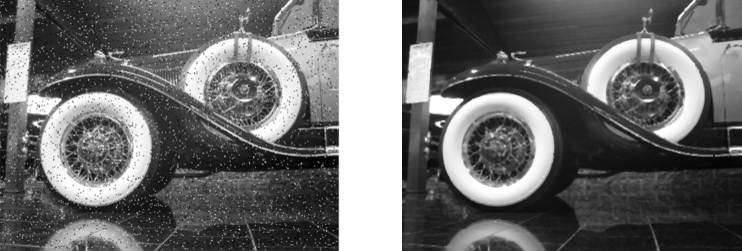
\includegraphics[width=9cm]{Figuras/Img04.png}

    \footnotesize
    \begin{tikzpicture}
    % Left matrix
    \matrix[matrix of nodes, nodes={draw, minimum size=0.8cm, anchor=center}, column sep=-\pgflinewidth, row sep=-\pgflinewidth] (A) {
        82 & 81 & 82\\
        81 & \color{purple}200 & 83 \\
        80 & 83 & 84 \\
    };
    
    % Green arrows pointing to the red value
    \foreach \i in {1,2,3} {
        \draw[->, thick, celeste, shorten >=-6pt, shorten <=-3pt] (A-\i-1) -- (A-2-2);
        \draw[->, thick, celeste, shorten >=-6pt, shorten <=-3pt] (A-\i-3) -- (A-2-2);
    }
    \foreach \i in {1,3} {
        \draw[->, thick, celeste, shorten >=-6pt, shorten <=-3pt] (A-\i-2) -- (A-2-2);
    }

    % Ordered list
    \node[draw, minimum height=0.8cm, right=4cm of A, anchor=center] (list) {
        \phantom{2}80 \quad 81 \quad 81 \quad 82 \quad \textcolor{celeste}{82} \quad 83 \quad 83 \quad 84 \quad 200
    };

    % Label 'Ordered List'
    \node[above=0.2cm of list] {Lista ordenada};

    % Arrow pointing to ordered list
    \draw[->, thick] (A) -- (list);

    % Arrow and label 'selected value'
    \draw[->, thick] (list.south) -- ++(0, -0.5) node[below] {valor seleccionado};

    % Right matrix
    \matrix[matrix of nodes, nodes={draw, minimum size=0.8cm, anchor=center}, right=8cm of A, column sep=-\pgflinewidth, row sep=-\pgflinewidth] (B) {
        \node {82}; & \node {81}; & \node {82}; \\
        \node {81}; & \node {\textcolor{celeste}{82}}; & \node {83}; \\
        \node {80}; & \node {83}; & \node {84}; \\
    };

    % Arrow pointing to right matrix
    \draw[->, thick] (list.east) -- (B);
\end{tikzpicture}

    \end{center}
\end{frame}

%%%%%%%%%%%%%%%%%%%%%%%%%%%%%%%%%%%%%%%%%%%%%%%%%%%%%%%%
\begin{frame}
    \frametitle{Un par más de conceptos}

    \begin{columns}
    \column{.5\textwidth}
    \begin{block}{Bounding Box}
        \begin{itemize}
            \item Delimita un objeto dentro de una imagen utilizando un rectángulo.
            \item Proporciona coordenadas $(x, y)$ y dimensiones $($ancho, alto$)$ del rectángulo.
        \end{itemize}
    \end{block}

    \column{.5\textwidth}

    \begin{tikzpicture}
    % Draw axes
    \draw[->, celeste] (-0.5,5) -- (4.5,5) node[right] {$x$};
    \draw[->, celeste] (0,5.5) -- (0,-0.5) node[right] {$y$};
    % (0,0) point and arrow
    \node[celeste, above left] at (0,5) {$(0,0)$};
    
    % Frame box
    \draw[thick, azul] (0,0) rectangle (4,5);
    
    % Bounding box
    \draw[thick, dashed] (1.5,3) rectangle (3,1);
    % (x,y) point and arrow
    \draw[dashed, celeste] (0,3) -- (1.5,3) -- (1.5,5);
    \fill[celeste] (1.5,3) circle (2pt);
    \node[celeste, above left] at (1.5,3) {$(x,y)$};
    
    \node at (2.25,2) {\scalebox{3.4}[5.2]{\color{azul}\faUmbrella}};
    \node[above right] at (1.5,3) {\footnotesize Bounding box};
    
    \draw[<->] (1.5,0.8) -- (3,0.8);
    \node[below] at (2.25,0.8) {\footnotesize ancho};
    
    \draw[<->] (3.2,1) -- (3.2,3);
    \node[right] at (3.2,2) {\rotatebox{90}{\footnotesize alto}};
    
    \end{tikzpicture}

    \end{columns}
    
\end{frame}
%%%%%%%%%%%%%%%%%%%%%%%%%%%%%%%%%%%%%%%%%%%%%%%%%%%%%%%%
%%%%%%%%%%%%%%%%%%%%%%%%%%%%%%%%%%%%%%%%%%%%%%%%%%%%%%%%
\begin{frame}
    \frametitle{Un par más de conceptos}

    \begin{columns}
    \column{.5\textwidth}
    \begin{block}{Segmentación Semántica}
        \begin{itemize}
            \item Asigna una etiqueta a cada píxel de la imagen, clasificándolos según el tipo de objeto al que pertenecen.
            \item Proporciona una delimitación precisa de los contornos de los objetos.
        \end{itemize}
    \end{block}
    \column{.5\textwidth}
    \begin{center}
        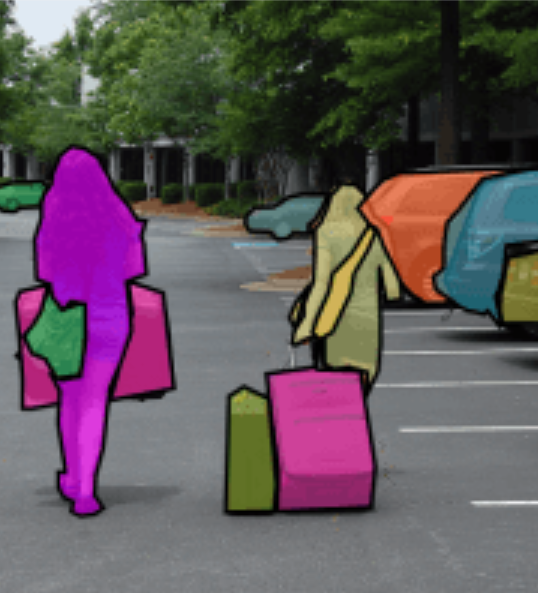
\includegraphics[width=5.5cm]{Figuras/Img05.png}
    \end{center}
    \end{columns}

\end{frame}
%%%%%%%%%%%%%%%%%%%%%%%%%%%%%%%%%%%%%%%%%%%%%%%%%%%%%%%%

%%%%%%%%%%%%%%%%%%%%%%%%%%%%%%%%%%%%%%%%%%%%%%%%%%%%%%%%
\begin{frame}
    \frametitle{¿Cómo aprende una máquina a interpretar una imagen?}

    \begin{block}{}
        \centering
        Una imagen no es más que una tabla de números. \\[0.4cm]
        ¿Cómo puede una computadora aprender, a partir de esos números, \\
        que está viendo una abeja, una mariposa o una flor?
    \end{block}

    \pause
    \vspace{0.4cm}
    \centering
    La respuesta: \textbf{redes neuronales convolucionales}.

\end{frame}
%%%%%%%%%%%%%%%%%%%%%%%%%%%%%%%%%%%%%%%%%%%%%%%%%%%%%%%%

%%%%%%%%%%%%%%%%%%%%%%%%%%%%%%%%%%%%%%%%%%%%%%%%%%%%%%%%
\fondo{celeste}
\section{Redes convolucionales}
\fondo{blanco}
%%%%%%%%%%%%%%%%%%%%%%%%%%%%%%%%%%%%%%%%%%%%%%%%%%%%%%%%


%%%%%%%%%%%%%%%%%%%%%%%%%%%%%%%%%%%%%%%%%%%%%%%%%%%%%%%%
\begin{frame}
    \frametitle{Redes convolucionales}

    \begin{itemize}
        \item Se inspiran en la corteza visual de los animales.
        \item Desarrollo desde Neocognitron (Fukushima, 1982) a LeNet-5 (LeCun, 1989).
        \item Avance impulsado por hardware mejorado y algoritmos optimizados a partir de 2012.
        \item CNNs aplican filtros convolucionales para extraer patrones como bordes, texturas, y formas a diferentes niveles de abstracción.
    \end{itemize}

    
\end{frame}
%%%%%%%%%%%%%%%%%%%%%%%%%%%%%%%%%%%%%%%%%%%%%%%%%%%%%%%%

%%%%%%%%%%%%%%%%%%%%%%%%%%%%%%%%%%%%%%%%%%%%%%%%%%%%%%%%
\begin{frame}
\centering
    \postitimg[12cm]{Figuras/FigDL.png}
\end{frame}
%%%%%%%%%%%%%%%%%%%%%%%%%%%%%%%%%%%%%%%%%%%%%%%%%%%%%%%%


%%%%%%%%%%%%%%%%%%%%%%%%%%%%%%%%%%%%%%%%%%%%%%%%%%%%%%%%
\begin{frame}
    \frametitle{Estructura de una Red Neuronal Convolucional (CNN)}

    \begin{itemize}[leftmargin=*]
        \item \textbf{Bloque convolucional:}
        \begin{itemize}[leftmargin=*]
            \item Incluye capas de convolución, agrupamiento (pooling) y activación.
            \item Detecta patrones y características en los datos de entrada.
        \end{itemize}

        \item \textbf{Bloque totalmente conectado:}
        \begin{itemize}[leftmargin=*]
            \item Cada neurona se conecta con todas las neuronas de la capa anterior y siguiente.
            \item Correlacionan las características detectadas por las capas convolucionales.
        \end{itemize}

        \item \textbf{Bloque de decisión:}
        \begin{itemize}[leftmargin=*]
            \item Genera un vector de probabilidades para cada clase.
            \item Usa funciones como softmax.
        \end{itemize}
    \end{itemize}

\end{frame}
%%%%%%%%%%%%%%%%%%%%%%%%%%%%%%%%%%%%%%%%%%%%%%%%%%%%%%%%


%%%%%%%%%%%%%%%%%%%%%%%%%%%%%%%%%%%%%%%%%%%%%%%%%%%%%%%%
\begin{frame}[fragile]
    \frametitle{Estructura de una Red Neuronal Convolucional (CNN)}

    \begin{center}
\tikzstyle{block} = [rectangle, draw, rounded corners, minimum width=1cm, minimum height=3cm, node distance=2cm]
\begin{tikzpicture}
    % Blocks
    \node (data) {Datos};
    \node (conv) [block, right of=data, fill=green!20] {\rotatebox{90}{Bloque Convolucional}};
    \node (fc) [block, right of=conv, fill=gray!20] {\rotatebox{90}{Bloque totalmente conectado}};
    \node (softmax) [block, right of=fc, fill=red!20] {\rotatebox{90}{Bloque de decisión}};
    \node[right=of softmax] (results) {Resultados};

    % Arrows
    \draw[->] (data) -- (conv);
    \draw[->] (conv) -- (fc);
    \draw[->] (fc) -- (softmax);
    \draw[->] (softmax) -- (results);

\end{tikzpicture}
    \end{center}
\end{frame}
%%%%%%%%%%%%%%%%%%%%%%%%%%%%%%%%%%%%%%%%%%%%%%%%%%%%%%%%


%%%%%%%%%%%%%%%%%%%%%%%%%%%%%%%%%%%%%%%%%%%%%%%%%%%%%%%%
\begin{frame}[fragile]
    \frametitle{Estructura de una Red Neuronal Convolucional (CNN)}

    \begin{center}\small
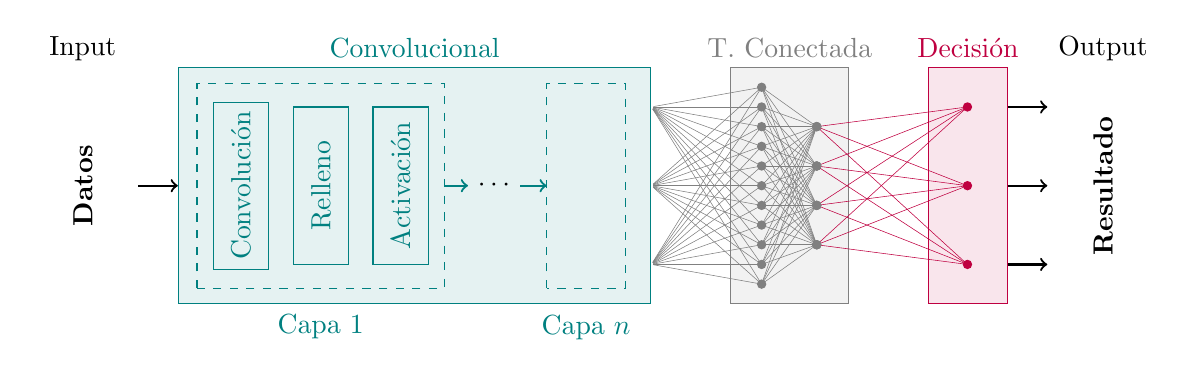
\begin{tikzpicture}
    % Data block (Input)
    \node[minimum height=2.9cm, label=above:Input, minimum width=1.4cm] (data) {\rotatebox{90}{\textbf{Datos}}};
    
    % Convolutional block
    \node[draw=teal, fill=teal!10, right=0.5cm of data, minimum width=6cm, minimum height=3cm, label={[text=teal]above:Convolucional}] (convblock) {};
    
    % FC block
    \node[draw=gray, fill=gray!10, right=1cm of convblock, minimum width=1.5cm, minimum height=3cm, label={[text=gray]above:T. Conectada}] (fc) {};
    
    % Softmax block
    \node[draw=purple, fill=purple!10, right=1cm of fc, minimum width=1cm, minimum height=3cm, label={[text=purple]above:Decisión}] (softmax) {};
    
    % Convolutional layers inside convolutional block
    \node[draw=teal, minimum width=0.7cm, minimum height=2cm] (conv) at ($(convblock.west)+(0.8,0)$) {\rotatebox{90}{\color{teal}Convolución}};
    \node[draw=teal, minimum width=0.7cm, minimum height=2cm, right=0.3cm of conv] (pool) {\rotatebox{90}{\color{teal}Relleno}};
    \node[draw=teal, minimum width=0.7cm, minimum height=2cm, right=0.3cm of pool] (act) {\rotatebox{90}{\color{teal}Activación}};

    % Capa 1
    \draw[dashed, color=teal] ($(conv.west)+(-0.2,-1.3)$) rectangle ($(act.east)+(0.2,1.3)$);
    \node[below=0.5cm of pool] {\color{teal}Capa 1};
    
    % Puntos
    \node[right=0.5cm of act] (dots) {$\cdots$};

    % Capa n
    \draw[dashed, color=teal] ($(act.east)+(1.5,-1.3)$) rectangle ($(act.east)+(2.5,1.3)$);
    \node at ($(act.east)+(2,-1.8)$) {\color{teal}Capa $n$};

    % Arrow connections Convolucional
    \draw[->, thick] (data.east) -- (convblock.west);
    \draw[->, thick, teal] ($(act.east)+(0.2,0)$) -- (dots.west);
    \draw[<-, thick, teal] ($(act.east)+(1.5,0)$) -- (dots.east);

    
    % FC connections
    \node (a1) at ($(convblock.east)+(0,1)$) [inner sep=0pt]{};
    \node (a2) at ($(convblock.east)$) [inner sep=0pt]{};
    \node (a3) at ($(convblock.east)+(0,-1)$) [inner sep=0pt]{};

    \foreach \i in {-1.25,-1,...,1.25} {
        \foreach \a in {a1, a2, a3} {
            \draw[line width=0.2pt, color=gray] (\a) -- ($(fc.west)+(0.4,+\i)$);
        }
        \foreach \j in {-0.75,-0.25,...,0.75} {
            \draw[line width=0.2pt, color=gray] ($(fc.west)+(0.4,+\i)$) -- ($(fc.west)+(1.1,+\j)$);
        }
        \node at ($(fc.west)+(0.4,+\i)$) [circle, fill=gray, inner sep=1.2pt]{};
    }
    
    \foreach \j in {1,0,-1} {
        \node at ($(softmax.west)+(0.5,+\j)$) [circle, fill=purple, inner sep=1.2pt]{};
        \foreach \i in {-0.75,-0.25,...,0.75} {
            \draw[line width=0.2pt, color=purple] ($(fc.west)+(1.1,+\i)$) -- ($(softmax.west)+(0.5,+\j)$);
            \node at ($(fc.west)+(1.1,+\i)$) [circle, fill=gray, inner sep=1.2pt]{};
        }
        \draw[->, thick] ($(softmax.east)+(0,\j)$) -- ++(0.5,0);
    
    }

    % Data block (Input)
    \node[minimum height=2.9cm, minimum width=1.4cm, label=above:Output, right=0.5cm of softmax] {\rotatebox{90}{\textbf{Resultado}}};
\end{tikzpicture}
    \end{center}
\end{frame}
%%%%%%%%%%%%%%%%%%%%%%%%%%%%%%%%%%%%%%%%%%%%%%%%%%%%%%%%


%%%%%%%%%%%%%%%%%%%%%%%%%%%%%%%%%%%%%%%%%%%%%%%%%%%%%%%%
\begin{frame}
    \frametitle{Ejemplo de una CNN: LeNet-5}
    
    \centering
    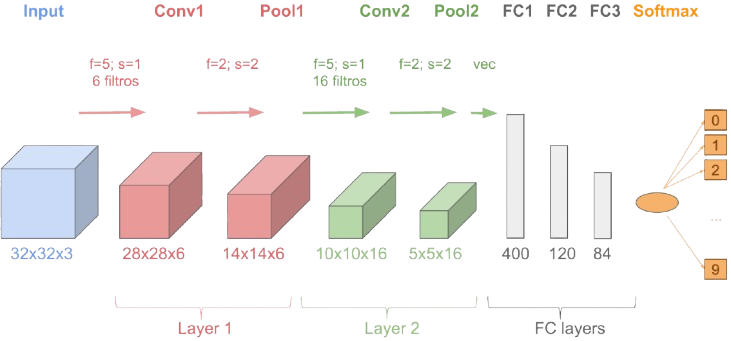
\includegraphics[width=0.9\linewidth]{Figuras/Img11.png}

\end{frame}
%%%%%%%%%%%%%%%%%%%%%%%%%%%%%%%%%%%%%%%%%%%%%%%%%%%%%%%%

%%%%%%%%%%%%%%%%%%%%%%%%%%%%%%%%%%%%%%%%%%%%%%%%%%%%%%%%
\begin{frame}
    \frametitle{Parámetros de LeNet-5}
    \centering
    \begin{tabular}{ccrr}
    \toprule
    \textbf{Capa}  & \textbf{Dimensión} & \textbf{Tamaño} & \textbf{Parámetros} \\
    \midrule
    Input   & $(32 \times 32 \times 3)$   & 3072   & 0        \\
    Conv1   & $(28 \times 28 \times 6)$   & 4704   & 456      \\
    Pool1   & $(14 \times 14 \times 6)$   & 1176   & 0        \\
    Conv2   & $(10 \times 10 \times 16)$  & 1600   & 2416    \\
    Pool2   & $(5 \times 5 \times 16)$    & 400     & 0        \\
    FC2     & $(120 \times 1)$       & 120     & 48120   \\
    FC3     & $(84 \times 1)$        & 84      & 10164   \\
    Softmax & $(10 \times 1)$        & 10      & 850      \\
    \midrule
    Total &&&62006\\
    \bottomrule
    \end{tabular}

\end{frame}
%%%%%%%%%%%%%%%%%%%%%%%%%%%%%%%%%%%%%%%%%%%%%%%%%%%%%%%%

%%%%%%%%%%%%%%%%%%%%%%%%%%%%%%%%%%%%%%%%%%%%%%%%%%%%%%%%
\begin{frame}
    \frametitle{Transferencia del Aprendizaje}

    \begin{itemize}[leftmargin=*]
        \item Permite reutilizar un modelo entrenado en una tarea para aplicarlo en otra tarea similar.
        \item Mejora el rendimiento del modelo y acelera el progreso.
        \item Es popular en \textbf{Deep Learning} debido a los altos costos computacionales y de datos necesarios para entrenar modelos desde cero.
        \item La técnica más común es usar un \textbf{modelo pre-entrenado} y adaptarlo:
        \begin{itemize}
            \item Seleccionar el modelo fuente.
            \item Reutilizar todo o parte del modelo.
            \item Ajustar el modelo a la nueva tarea (fine-tuning).
        \end{itemize}
    \end{itemize}

\end{frame}
%%%%%%%%%%%%%%%%%%%%%%%%%%%%%%%%%%%%%%%%%%%%%%%%%%%%%%%%

%%%%%%%%%%%%%%%%%%%%%%%%%%%%%%%%%%%%%%%%%%%%%%%%%%%%%%%%
\begin{frame}
    \frametitle{¿Y en la práctica?}

    \begin{block}{}
        \centering
        Con redes convolucionales y transferencia del aprendizaje disponemos
        de herramientas muy poderosas para analizar imágenes.
    \end{block}

    \pause
    \vspace{0.4cm}
    \begin{alertblock}{}
        \centering
        Con esta ideas, podemos \textbf{detectar polinizadores en imágenes de flores}.
    \end{alertblock}

\end{frame}
%%%%%%%%%%%%%%%%%%%%%%%%%%%%%%%%%%%%%%%%%%%%%%%%%%%%%%%%

% --- Trabajo de investigación ---
\include{Secciones/03Implementacion}
\include{Secciones/04Conclusiones}

%%%%%%%%%%%%%%%%%%%%%%%%%%%%%%%%%%%%%%%%
%% Página final
\fondo{final}
\begin{frame}[plain]
\begin{center}
    \color{white}

    \vspace{1.5cm}
    {\Huge\textbf{Gracias}}
    \vspace{2mm}


    \begin{tabular}{ccc}
        \color{azul!60!black}\qrcode[hyperlink,height=2.5cm]{https://linktr.ee/aemerinot}
        &\phantom{.\hspace{.5cm}.}&
        \color{azul!60!black}\qrcode[hyperlink,height=2.5cm]{https://github.com/andres-merino/Presentacion-ChatGPT-AulaInvertida}
        \\[1.3cm]
        \LARGE \faLinkedin\hspace{5mm} \faGithub%\hspace{5mm} \aiOrcidSquare
        &&
        Presentación
    \end{tabular}

    \vspace{2mm}
    \textbf{Contacto:} aemerinot@puce.edu.ec
\end{center}
\end{frame}


\end{document}
